\header{
    \section{L'apéro et l'impétrant} \label{l-apero-et-l-impetrant}
    %
    \insertComment{Sur l'air de l'oiseau et l'enfant}{Paroles de Yanis Ingénieur Grenoble}
}

\enluminure{4}{\href{}{C}}{omme} l'impétrant, qui finit son verre
\\Qui voit passer au loin l'apéro
\\Comme l'apéro, où il se ressert
\\Vois comme le monde, le monde est beau
\\\\Beau, mon Parrain-e, et ses propos vagues
\\Ivre de bière, de vin et de chant
\\Bel-le Marrain-e, qui aussi divague
\\Trop déchiré-e dans ses draps blancs
\\\\Blanche, rouge ou blonde, en verre ou en pinte
\\Comptoir de vie, tireuse d'amour
\\Remplis ma vie, je bois sans étreinte
\\Remplis mon verre, encore un tour
\\\\Tour des bungal's, faluchard avachi
\\Qui veut reboire, mon dieu qu'il est lourd
\\Où mon/ma GM, décernant son pachi
\\Peut nous donner, un monde d'amour
\\\\L'alcool c'est toi
\\L'alcool c'est moi
\\L'oisif c'est toi
\\L'envie c'est moi
\\\\Moi je ne suis qu'impétrant-e de longue
\\Qui doit attendre devant le comptoir
\\Toi mon comptoir, qui remplis mon ventre
\\C'est le dernier, juste pour ce soir
\\\\Soir, la galère, je tombe par terre
\\Je bois de l'eau, je rentre en chantant
\\Pensant à mon potentiel baptême
\\Être faluchard-e ou impétrant
\breakpage
\\\\Comme l'impétrant, qui finit son verre
\\Qui voit passer au loin l'apéro
\\Comme l'apéro, où il se ressert
\\Mon baptême arrivera un jour
\\\\L'alcool c'est toi
\\L'alcool c'est moi
\\L'oisif c'est toi
\\L'envie c'est moi
\\L'oisif c'est toi
\\L'envie c'est moi
\\L'oisif c'est toi
\\L'envie c'est moi

\vspace{1cm}
\begin{center}
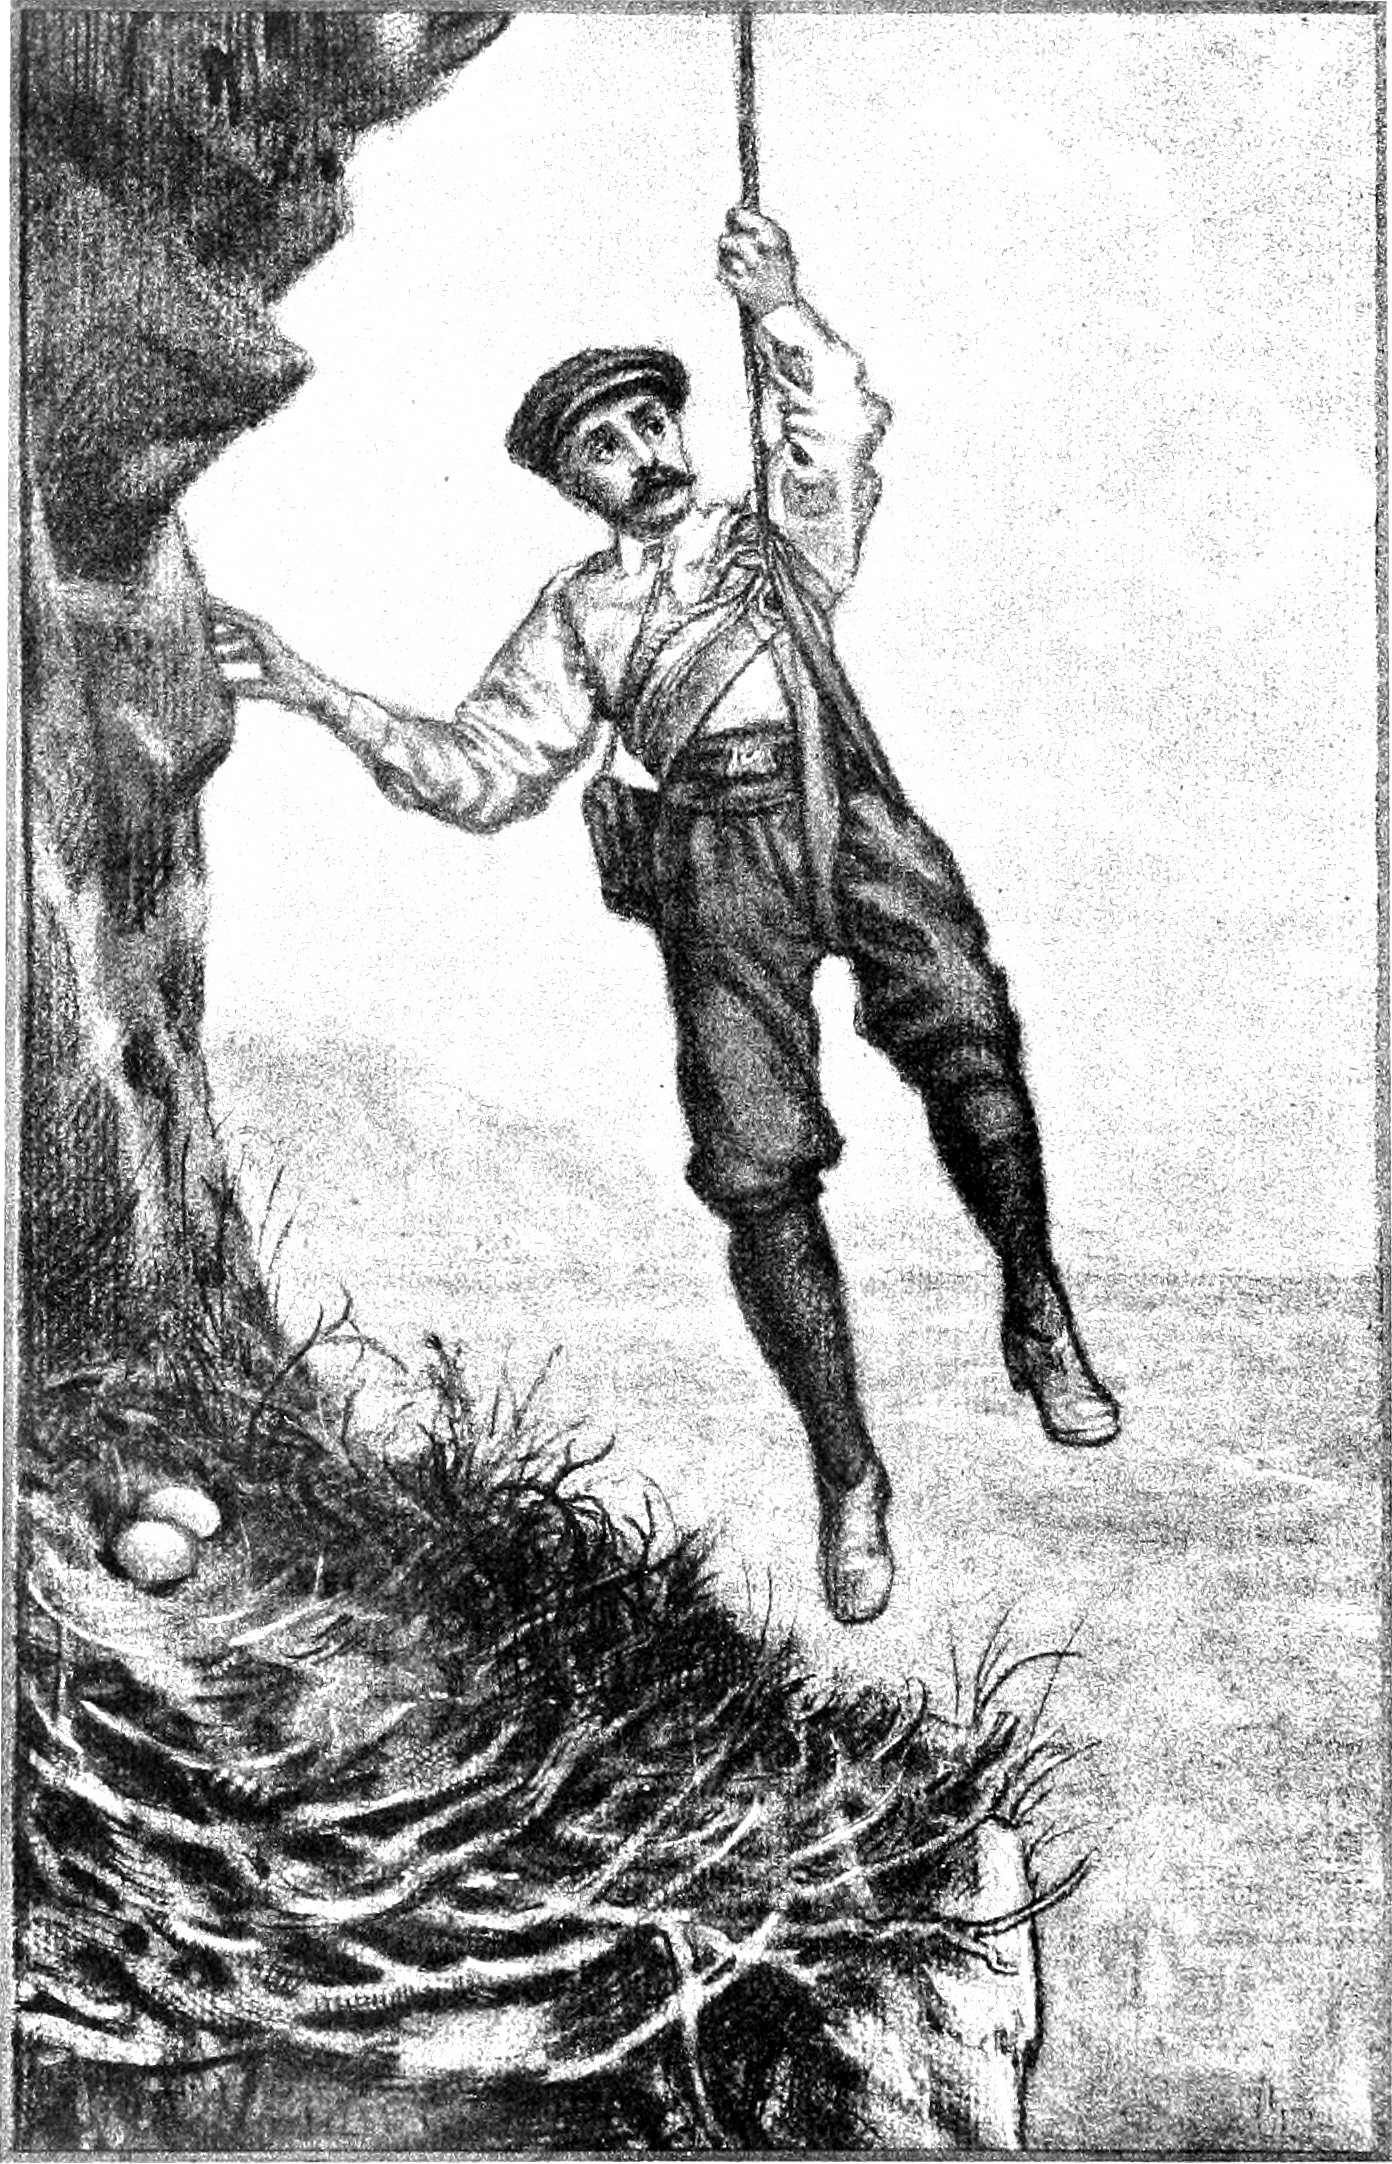
\includegraphics[width=0.6\textwidth]{images/brev23.png}
\end{center}

\breakpage